\documentclass[hyperref={dvipdfmx,pdfpagelabels=false}]{beamer}
\title{Einführung in Matlab - Einheit 4}
\subtitle{Visualisieren, Datenstrukturen, In- und Output, Etwas Debugging}
\mode<article>
{
  \usepackage{fullpage}
  \usepackage{pgf}
  \usepackage{hyperref}
  \setjobnamebeamerversion{beamer}
}

\mode<presentation>
{
  %\usetheme{Frankfurt}
 %\usetheme{My}
  \usetheme{Madrid}
  % or ...
%\usecolortheme{seagull}
  %\setbeamercovered{transparent}
  %\setbeamercovered{dynamic}
  % or whatever (possibly just delete it)
}
\usenavigationsymbolstemplate{}
\usefonttheme{structurebold}
\usepackage{multimedia}
\usepackage{tikz}
\usepackage{fontspec,xunicode,xltxtra}
%\usepackage[scaled=.90]{helvet}
% Or whatever. Note that the encoding and the font should match. If T1
% does not look nice, try deleting the line with the fontenc.

\setbeamertemplate{footline}
{
\leavevmode
%\hbox{\begin{beamercolorbox}[wd=.5\paperwidth,ht=2.5ex,dp=1.125ex,
%leftskip=.3cm plus1fill,rightskip=.3cm]{author in head/foot}%
%    \usebeamerfont{author in head/foot}\insertshortauthor
%  \end{beamercolorbox}%
%  \begin{beamercolorbox}[wd=.5\paperwidth,ht=2.5ex,dp=1.125ex,leftskip=.3cm,
%rightskip=.3cm plus1fil]{title in head/foot}%
%    \usebeamerfont{title in head/foot}\insertshorttitle\hfill

\hfill\insertframenumber  \hspace{3pt}

%\inserttotalframenumber
%\hspace*{2ex}
%  \end{beamercolorbox}}%
  \vskip3pt%
}

%\usepackage[english]{babel}
\usepackage[ngerman]{babel}
\selectlanguage{ngerman}

%
% math/symbols
%
\usepackage{amssymb}
\usepackage{amsthm}
% \usepackage{latexsym}
\usepackage{amsmath}
%\usepackage{listings}
\usepackage[framed]{mcode}
%\usepackage{mcode}

\usepackage{mydef}
\usepackage{cmap} % you can search in the pdf for umlauts and ligatures
%\usepackage{colonequals} %corrects the definition-symbols \colonequals (besides others)
\title{Einführung in Matlab}
%
%\subtitle{Disputation} % (optional)

\author{Jochen Schulz}
% - Use the \inst{?} command only if the authors have different
%   affiliation.

\institute{Georg-August Universit\"at G\"ottingen \pgfimage[height=0.5cm]{../figures/unilogo3}}
% - Use the \inst command only if there are several affiliations.
% - Keep it simple, no one is interested in your street address.

\date{\today}

\subject{Einführung in Matlab}
% This is only inserted into the PDF information catalog. Can be left
% out. 



% If you have a file called "university-logo-filename.xxx", where xxx
% is a graphic format that can be processed by latex or pdflatex,
% resp., then you can add a logo as follows:

%\logo{\pgfimage[height=0.5cm]{figures/unilogo3}}


% Delete this, if you do not want the table of contents to pop up at
% the beginning of each subsection:
% \AtBeginSubsection[]
% {
%   \begin{frame}<beamer>
%     \frametitle{Aufbau}
%     \tableofcontents[currentsection,currentsubsection]
%   \end{frame}
% }

\AtBeginSection[]
{
  \begin{frame}<beamer>
    \frametitle{Aufbau}
    \tableofcontents[currentsection,currentsubsection]
  \end{frame}
}


\begin{document}



\maketitle

\section{Visualisieren von 3D-Daten}

%
% Slide
% 
\begin{frame}[fragile]\frametitle{Problem}
\begin{itemize}
\item Daten liegen h\"aufig in Form von Vektoren $(x,y,z)$ vor. Man m\"ochte
  eine Funktion $F$ mit $z(i)=F(x(i),y(i))$ plotten.
\item Befehle \mcode{surf} und \mcode{mesh} funktionieren nur wenn  die
  Einträge in $x$ und $y$ monoton sind und die Daten auf einem kartesischen
  Gitter vorliegen.
\item Ausweg: Interpolieren der Daten auf ein entsprechendes Gitter. 
\end{itemize}
\end{frame}
%
% Slide
% 
\begin{frame}[fragile]\frametitle{Beispiel}
\begin{lstlisting}
load seamount
plot(x,y,'.','markersize',10)
figure, plot3(x,y,z,'.')
\end{lstlisting}
\begin{center}
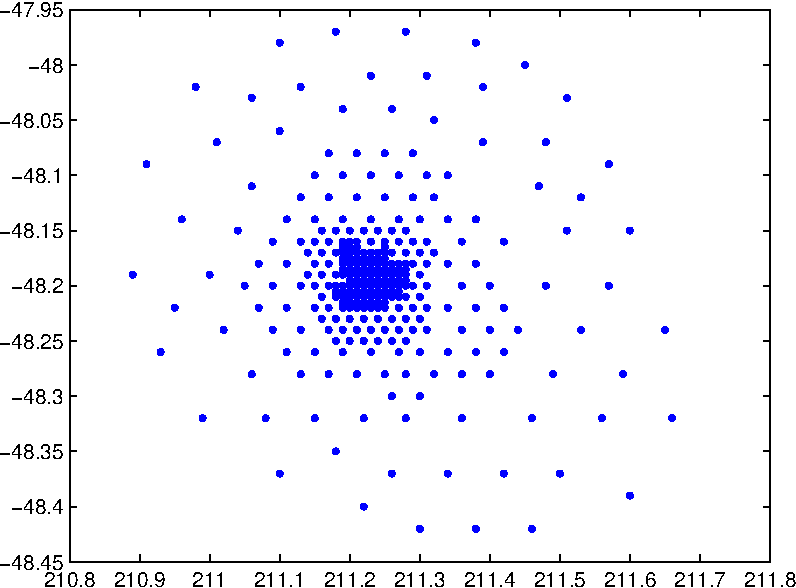
\includegraphics[width=0.6\textwidth]{figures/beispiel_scattered_data}
\end{center}
\end{frame}
%
% Slide
% 
\begin{frame}[fragile]\frametitle{Beispiel}
\begin{lstlisting}
xi = linspace(min(x),max(x),40);
yi = linspace(min(y),max(y),40);
[XI,YI] = meshgrid(xi,yi);
F = TriScatteredInterp(x,y,z,'linear');
ZI = F(XI,YI);
surf(XI,YI,ZI)
\end{lstlisting}
\begin{center}
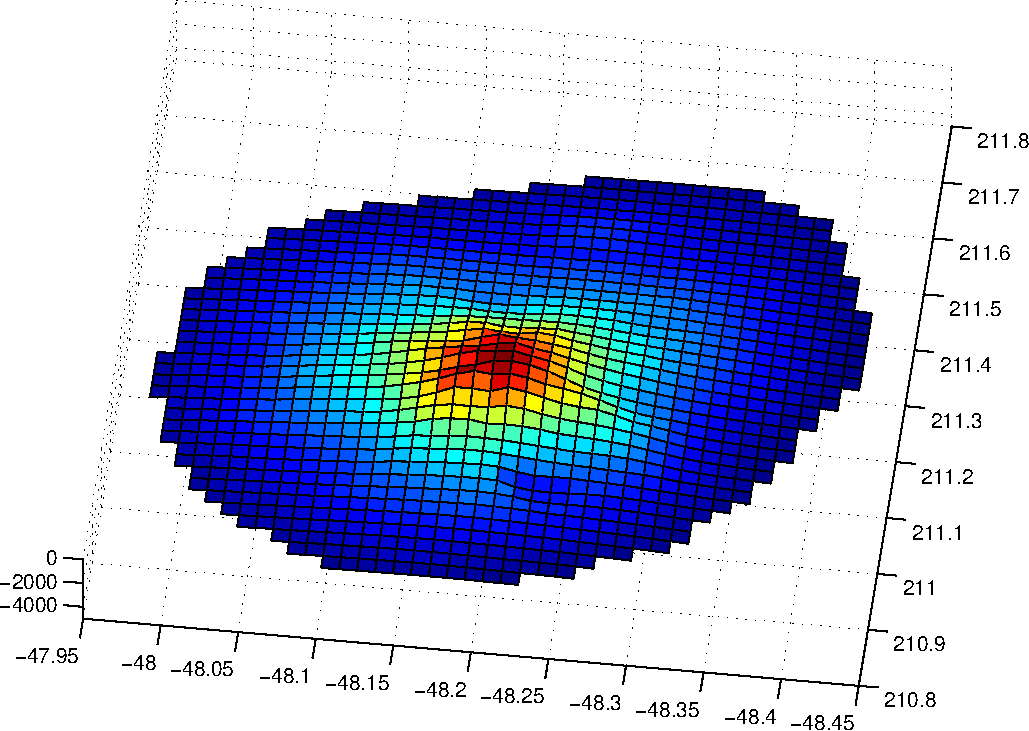
\includegraphics[width=0.6\textwidth]{figures/beispiel_scattered_data_plot}
\end{center}
\end{frame}
%
% Slide
% 
\begin{frame}[fragile]\frametitle{griddata}
\begin{lstlisting}
F = TriScatteredInterp(<x>,<y>,<z>,<methode>);
ZI = F(<XI>,<YI>);
\end{lstlisting}
\begin{itemize}
\item Vektoren $x,y,z$ enthalten Werte $(x(i),y(i),z(i))$.
\item Interpolationsstellen $(XI(i,j),YI(i,j))$ mit Matrizen \mcode{XI, YI}. 
\item Funktionsauswertung mit \mcode{F}: Ergebnis $ZI(i,j)$.
\item Art des Interpolierens:
\begin{itemize}
 \item \mcode{'nearest'}: st\"uckweise konstant
 \item \mcode{'linear'}: linear
 \item \mcode{'natural'}: natürliche Nachbarn (Voronoi-Diagramm)
\end{itemize}
\item Es wird nur innerhalb der konvexen H\"ulle der Punkte $(x(i),y(i))$
  interpoliert. Ansonsten Funktionswert \mcode{NaN}. 
\end{itemize}
\end{frame}

%
% Slide
% 
\begin{frame}[fragile]\frametitle{Bemerkungen}
\begin{itemize}
\item Der Interpolation liegt eine Delaunay Triangulation zugrunde. Die Werte
  $(x(i),y(i))$ sind Eckpunkte der entstehenden Dreiecksmenge.
\item Danach werden mit Hilfe der Dreiecke Funktionen  definiert, die
  entsprechende Werte besitzen. 
\item Mittels \mcode{TriScatteredInterp} ist die Technik auch auf h\"ohere Dimensionen
  anwendbar. Dreiecke werden durch entsprechende höher-dimensionale
  Simplizes ersetzt. \\
(In 3D Tetraeder)
\end{itemize}
\end{frame}
%
% Slide
% 
\begin{frame}[fragile]\frametitle{interp2}
\begin{lstlisting}
ZI = interp2(<X>,<Y>,<Z>,<XI>,<YI>,<methode>)
\end{lstlisting}
\begin{itemize}
\item Allgemein sind $X,Y,Z$ Matrizen. Dabei ist $Z(i,j)$ der Funktionswert an
  $(X(i,j),Y(i,j))$. $X$ und $Y$ sind in der Regel durch \mcode{meshgrid} erzeugt. 
\item Es wird an den Stellen $(XI(i,j),YI(i,j))$ interpoliert. Das Ergebnis
  ist $ZI(i,j)$. Die Einträge von $XI$ bzw. $YI$ k\"onnen beliebig sein. 
\item Die Art des Interpolierens ist entweder \mcode{'nearest'}, \mcode{'linear'}
  oder \mcode{'cubic'}. 
%Entsprechend wird entweder st\"uckweise konstant, linear
%  oder durch bikubische Splines interpoliert. 
\end{itemize}
\end{frame}

\section{Datenstrukturen}
%
%
%
\begin{frame}[fragile]\frametitle{Datenstrukturen}
\begin{itemize}
\item In MATLAB gibt es verschiedene {\it Datentypen}. 
Sie werden bestimmt durch ihre Eigenschaften.
\item Einzelne Elemente eines Datentyps werden {\it Objekte} genannt. 
\item Ein {\it Objekt} besteht meist aus drei Teilen: {\it Bezeichner}, {\it
Referenzen} und {\it Werte} des Objekts.  
\item {\it Variablen} sind Datenobjekte deren Werte w\"ahrend eines
Programmablaufs ver\"andert werden k\"onnen. 
\end{itemize}
\end{frame}
%
%
%
\begin{frame}[fragile]\frametitle{Datentypen in MATLAB}
\begin{itemize}
\item MATLAB speichert alle Variablen als Felder. Ein Skalar ist eine $1 \times
1$-Matrix. 
\item MATLAB weist den Datentyp {\it implizit} zu. Durch die Zuweisung eines
Wertes wird der Typ implizit bestimmt. 
\item Den Datentyp eines Objekts $a$ kann durch den Befehl \alert{
\mcode{class(a)}} bestimmt werden.
\end{itemize}
\end{frame}
%
%
%
\begin{frame}[fragile]\frametitle{Datentypen in MATLAB}
\begin{itemize}
\item Gleitkommazahlen (Komplexe Zahlen)
\item Characters und Strings
\item Strukturen
\item Cell Arrays
\item Funktionen
\item Sparse Matrizen
\item Integer-Zahlen
\item Logische Ausdr\"ucke
\end{itemize}
\end{frame}
%
% Folie
%
\begin{frame}[fragile]\frametitle{Gleitkommazahlen}
\begin{itemize}
\item Standard-Datentyp ist ein Array von Gleitkommazahlen (\mcode{double}).
\item Abstand von $1$ zur nächsten Gleitkommazahl in MATLAB: $\epsilon
  =2^{-52}$ (vgl. \mcode{eps} in MATLAB)
\item Sei $x \in \mathbb{R}$ eine reelle Zahl und $\tilde x$ die
  Darstellung in MATLAB. Dann gilt für den Rundungsfehler \\[-0.5cm]
\[ \frac{|x - \tilde x|}{|x|}\leq \frac{1}{2} \epsilon .\]
\item Die größte bzw. kleinste in MATLAB darstellbare positive Zahl
  ist in
\mcode{realmin} bzw. \mcode{realmax} gespeichert. 
\end{itemize}
\end{frame}
%
% Folie
%
\begin{frame}[fragile]\frametitle{Ausnahmen}
\begin{itemize}
\item Ist eine Zahl größer als \mcode{realmax}, so meldet MATLAB einen
  'Overflow' und gibt als Ergebnis \mcode{Inf} zurück.
\begin{lstlisting}
realmax*1.1
\end{lstlisting}
\begin{matlab}
 ans =   Inf
\end{matlab}

\item Bei Operationen wie $0/0$  oder $\infty / \infty$, erhält man als Ergebnis
  \mcode{NaN} ({\it Not a Number}).
\begin{lstlisting}
0/0 
\end{lstlisting}
\begin{matlab}
Warning: Divide by zero.
ans =   NaN 
\end{matlab}

\end{itemize}
\end{frame}
%
% Folie
%
\begin{frame}[fragile]\frametitle{Umgang mit NaN und       Inf  }
\begin{itemize}
\item Mit Hilfe von \alert{ \mcode{isinf}} und \alert{ \mcode{isnan}} kann auf
$\infty$ bzw. NaN getestet werden.
 \begin{lstlisting}
isnan(0/0), isinf(1.2*realmax)
\end{lstlisting}
\begin{matlab}
ans =   1  ans =   1
\end{matlab}
\item Test auf NaN durch $==$ ist nicht m\"oglich
\begin{lstlisting}
0/0 == NaN
\end{lstlisting}
\begin{matlab}
ans =     0
\end{matlab}
\item Bei Inf ist der Test durch $==$  m\"oglich!
\begin{lstlisting}
(1.2*realmax)==Inf
\end{lstlisting}
\begin{matlab}
ans =     1
\end{matlab}
\end{itemize}
\end{frame}
%
% Folie
%
\begin{frame}[fragile]\frametitle{Single}
\begin{itemize}
\item \"Ahnlich wie in C gibt es den Datentyp \mcode{single}. Es ist eine
Darstellung in geringerer Genauigkeit. 
\item Durch den Befehl \alert{ \mcode{single()}} wird eine \mcode{double}-Zahl in
eine \mcode{single}-Zahl konvertiert. 
\item Arithmetische Operationen mit \mcode{double}- und \mcode{single}-Objekten
ergeben  \mcode{single}-Objekte.
\end{itemize}
\end{frame}
%
% Folie
%
\begin{frame}[fragile]\frametitle{Single}
\begin{lstlisting}
a = sqrt(2); b = single(a);
c = a+b; d = a-b
\end{lstlisting}
\begin{matlab}
d =
  2.4203e-08
\end{matlab}
\begin{lstlisting}
whos
\end{lstlisting}
\begin{matlab}
  Name   Size     Bytes  Class    
  a      1x1        8  double              
  b      1x1        4  single              
  c      1x1        4  single              
  d      1x1        4  single  
\end{matlab}
\begin{lstlisting}
[realmax, single(realmax)], realmax
\end{lstlisting}
\begin{matlab}
ans =
   Inf   Inf
ans =
  1.7977e+308
\end{matlab}
\end{frame}
%
% Folie
%
\begin{frame}[fragile]\frametitle{Operator Rangfolge}
\begin{tabular}{|cp{10cm}|}
\hline
Level & Operator\\
\hline
1 &   Exponent (\mcode{^}, \mcode{.^}), \mcode{transpose}\\
2 & logische Verneinung (\mcode{\~})\\
3 & Multiplikation (*,.*), Division (\mcode{/},\mcode{./},\mcode{\\}, \mcode{.\\})\\
4 & Addition (+), Subtraktion (-)\\
5 & Doppelpunktoperator (:)\\
6 & Vergleichsoperatoren (\mcode{<},\mcode{>},\mcode{<=},\mcode{>=},\mcode{==},\mcode{\~=})\\ 
7 & Logisches und (\mcode{\&})\\
8 & Logisches oder (\mcode{|})\\
\hline
\end{tabular}\\[0.5cm]
{\scriptsize Bei gleicher Rangfolge wertet MATLAB von links nach rechts
  aus. \\
Die Rangfolge kann durch Klammersetzung geändert werden.}

\end{frame}
%
% Folie
%
\begin{frame}[fragile]\frametitle{Darstellungsformate am Beispiel $1/7$}
\begin{tabular}{ll}
\alert{ \mcode{format short}} &  0.1429 \\
\alert{ \mcode{format short e} }& 1.4286e-01\\
\alert{ \mcode{format short g} }&0.14286\\
\alert{ \mcode{format long} }& 0.14285714285714\\
\alert{ \mcode{format long g} }& 0.142857142857143\\
\alert{ \mcode{format long e} }& 1.428571428571428e-01\\
\end{tabular}

Das Default-Format ist \mcode{short}. 
\end{frame}
%
% Folie
%
\begin{frame}[fragile]\frametitle{Komplexe Zahlen}
Komplexe Zahlen $z \in \mathbb{C}$ haben die Form
\[ z = x +iy, \quad x,y \in \mathbb{R} \]
mit $i=\sqrt{-1}$. 
\begin{itemize}
\item $\sqrt{-1}$ ist in MATLAB vordefiniert in den Variablen $i$,$j$.
\item Durch \mcode{complex(x,y)}  kann aus $x,y \in
  \mathbb{R}$ die komplexe Zahl $x + iy$ erzeugt werden.
\item Für $z=x+iy \in \mathbb{C}$ erhält man den Realteil mit
  $real(z)$ und den Imaginärteil durch $imag(z)$. 
\end{itemize} 
\end{frame}
\begin{frame}[fragile]\frametitle{Polarkoordinaten}
\alert{ \[ z \in \mathbb{C}, \quad z=re^{i \varphi}=r(\cos \varphi + i \sin
  \varphi) \]}
\begin{itemize}
\item \mcode{abs(z)} ergibt den Betrag $r$ von $z$.
\item $\varphi$ erhält man durch \mcode{angle(z)}.
\item grafische Darst.:  \mcode{compass(z)} ($z=3+3i$). \\
 \centering{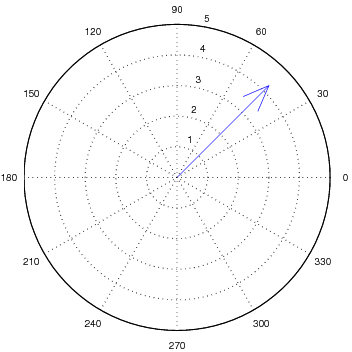
\includegraphics[width=0.3\textwidth]{../figures/kompass}}\\ 
\end{itemize}
\end{frame}

%
% Folie
%
\begin{frame}[fragile]\frametitle{Structures}
\alert{Structures:}\\
Strukturen sind eine Möglichkeit verschiedene Objekte in einer
Datenstruktur zu bündeln.\\[1cm]

\alert{Beispiel:} komplexe Zahlen
\begin{lstlisting}
komp_Zahl.real=1;
komp_Zahl.imag=1;
komp_Zahl
\end{lstlisting}
\begin{matlab}
komp_Zahl = 

    real: 1
    imag: 1
\end{matlab}
\end{frame}
%
% Folie
%
\begin{frame}[fragile]\frametitle{Structures II}
\begin{itemize}
\item Alternativ können Strukturen durch
\begin{lstlisting}
struktur = struct('Feld1',<Wert1>,'Feld2',<Wert2>,..)
\end{lstlisting}
definiert werden.
\item Ein Feld einer Struktur \mcode{struktur} kann durch 
\begin{lstlisting}
struc2 = rmfield( <struktur> ,'Feld')
\end{lstlisting}
gel\"oscht werden. 
\end{itemize}
\end{frame}
%
% Folie
%
\begin{frame}[fragile]\frametitle{Cell Arrays}
\alert{Cell Arrays:} \\
Cell Arrays sind spezielle Matrizen, deren  Einträge aus unterschiedlichen
Datentypen bestehen können. Erzeugt
werden sie durch geschweifte Klammern.\\
\begin{lstlisting}
C = { 1:10, hilb(4);...
       'Hilbert Matrix', pi}
\end{lstlisting} 
\begin{matlab}
C = 
       [1x10 double]    [4x4 double]
    'Hilbert Matrix'    [    3.1416]
\end{matlab} 
\end{frame}
%
% Folie
%
\begin{frame}[fragile]\frametitle{Befehle für Cell Arrays}
\begin{itemize}
\item Zugriff auf Cell-Arrays:\\ 
\begin{columns}[c]
\column{0.45\textwidth}
\begin{lstlisting} 
C{2,1}
\end{lstlisting}
\begin{matlab}
ans =
Hilbert Matrix
\end{matlab}
\column{0.45\textwidth}
\begin{lstlisting}
C{1,2}(2,3)
\end{lstlisting}
\begin{matlab}
ans =
    0.2500
\end{matlab}
\end{columns}
\item Durch \mcode{celldisp(C)} wird der Inhalt von $C$ dargestellt.
%\item \mcode{struct2cell} bzw. \mcode{num2cell} erzeugt ein Cell Array
%  aus einer Struktur bzw. einer normalen Matrix.
\item \mcode{cellplot(C)} stellt $C$ grafisch dar.
\end{itemize}
\end{frame}
%
% Folie
%
\begin{frame}[fragile]\frametitle{Integer}
\begin{itemize}
\item In diesen Datentypen werden ganze bzw. nat\"urliche Zahlen gepeichert.  
\item Zur effizienten Speicherung gibt es die Datentypen \mcode{int8},
\mcode{uint8}, \mcode{int16}, \mcode{uint16}, \mcode{uint16}, \mcode{int32},
\mcode{uint32}, \mcode{int64}, \mcode{uint64}. 
\item In den Datentypen, die mit \mcode{u} beginnen, werden nat\"urliche Zahlen
gespeichert, sonst ganze Zahlen.
\item Die abschlie{\ss}ende Zahl gibt den Speicherbedarf an. \mcode{uint8}
ben\"otigt z.B. $8$-Bit. (Wertebereich $0 \dots 2^8-1$).
\end{itemize}
\end{frame}
%
% Folie
%
\begin{frame}[fragile]\frametitle{Integer}
\begin{lstlisting}
a = int8(20); b = int16(20); c = int8(20);
a*c, a*b
\end{lstlisting}
\begin{matlab}
ans =  127
??? Error using ==> mtimes
Integers can only be combined with integers
of the same class, or scalar doubles.
\end{matlab}
\begin{lstlisting}
a+0.2
\end{lstlisting}
\begin{matlab}
ans =   20
\end{matlab}
\begin{lstlisting}
a+0.5
\end{lstlisting}
\begin{matlab}
ans =   21
\end{matlab}
\begin{lstlisting}
a*1.54
\end{lstlisting}
\begin{matlab}
ans =   31
\end{matlab}
\end{frame}
%
%
%
\section{In- und Output}
%
% Slide
%
\begin{frame}[fragile]\frametitle{Input und Output}
\begin{itemize}
\item Benutzereingabe
\item einfache und formatierte Ausgabe
\item Schreiben in Dateien
\item Einlesen von Daten aus Dateien
\item Speichern und Laden von Variablen\\
\item Durch \alert{ \mcode{help iofun}} erhält man eine Übersicht aller Ein- und
  Ausgabe - Befehle
\end{itemize}
\end{frame}
%
% Slide
%
\begin{frame}[fragile]\frametitle{Benutzereingabe}
\begin{itemize}
\item Standardeingabe: 
\begin{lstlisting}
input 
\end{lstlisting}
%\item Eingabe eines Zeichens:
\item Informationssteuerung durch die Maus:
\begin{lstlisting}
ginput 
\end{lstlisting}

\item Anhalten der Prozedur bis eine Tastatureingabe erfolgt: 
\begin{lstlisting}
pause
\end{lstlisting}

\end{itemize}
\end{frame} 
%
% Slide
%
\begin{frame}[fragile]\frametitle{input}
Die Benutzereingabe kann durch den Befehl \mcode{input('Text')} erfolgen. Es
wird der 'Text'  angezeigt. Die Eingabe kann hinter 'Text' erfolgen
und wird durch Return
abgeschlossen.  Durch die Option 's' wird ein String abgefragt.
  
\begin{lstlisting}
startwert = input('Bitte geben Sie den Startwert ein: ')
\end{lstlisting}
\begin{matlab}
Bitte geben Sie den Startwert ein: 56
 startwert =
     56

\end{matlab}
\begin{lstlisting}
f = input('Eingabe einer Funktion: ', 's')
\end{lstlisting}
\begin{matlab}
Eingabe einer Funktion: sin(x)*cos(x)
f =
sin(x)*cos(x)
\end{matlab}
\end{frame}
%
% Slide
%
\begin{frame}[fragile]\frametitle{ginput}
Das Kommando 
\begin{lstlisting}
[x,y]=ginput(n)
\end{lstlisting}
gibt die Vektoren $x$ und $y$ der Koordinaten der nächsten $n$
Maus-Klicks zurück, an denen sich die Maus im aktuellen Grafik-Fenster
befindet.  
\begin{itemize}
\item \mcode{[x,y]=ginput} sammelt so lange Daten ein, bis die
  Return-Taste gedrückt wird.
\item \mcode{[x,y,taste]=ginput(n)} gibt auch den Vektor \mcode{taste}
  zurück, der aus Werten $1$ (linke Maustaste), $2$ (mittlere
  Maustaste) oder $3$ (rechte Maustaste) besteht. 
\end{itemize} 
\end{frame}
%
% Slide
%
\begin{frame}[fragile]\frametitle{Bezier-Polynom}
\alert{ \[ z (t):=\sum_{i=0}^n {\bf b}_i B_i^n(t), \quad t \in [0,1] \]}
\begin{itemize}
\item $z(t): [0,1] \rightarrow \mathbb{R}^2$ ist das {\it Bezier-Polynom}.
\item ${\bf b}_i \in \mathbb{R}^2$ sind die vorgegebenen 
{\it Kontrollpunkte}.
\item $B_i^n(t)=\left( n \atop i \right) t^i (1-t)^{n-i}$ sind 
{\it Bernstein-Polynome}.
\end{itemize}
\end{frame}
%
% Slide
%
\begin{frame}[fragile]\frametitle{Bezier-Polynom}
\begin{center}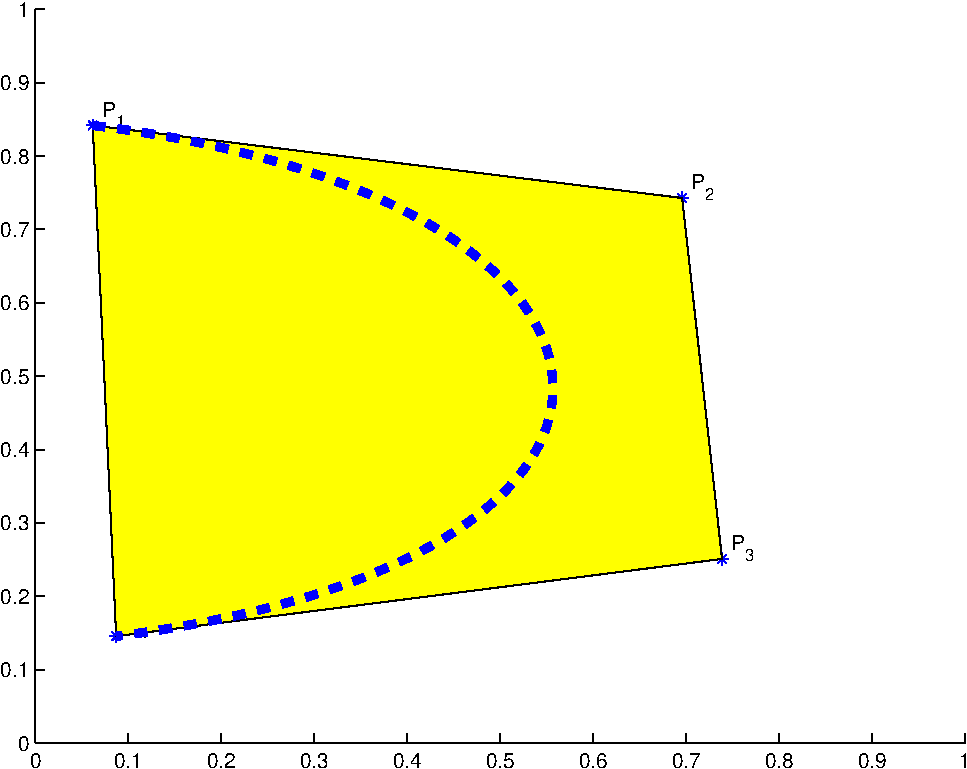
\includegraphics[width=0.8\textwidth]{figures/bezier}\end{center}
\end{frame}
%
% Slide
%
\begin{frame}[fragile]\frametitle{Bezier-Polynom}
\lstinputlisting{bezier.m}
\end{frame}
%
% Slide
%
\begin{frame}[fragile]\frametitle{Ausgabe}
\begin{itemize}
\item Angeben einer Variable ohne Semicolon:
\begin{lstlisting}
text=['Pi mit 5 signifikanten Stellen : ' num2str(pi,6)]
\end{lstlisting} 
\begin{matlab} 
text =
Pi mit 5 signifikanten Stellen : 3.14159
\end{matlab} 
\item Ausgabe des Strings $X$ durch  \mcode{disp(X)}
\begin{lstlisting}
disp(text)
\end{lstlisting} 
\begin{matlab} 
Pi mit 5 signifikanten Stellen : 3.14159
\end{matlab} 
\item Ausgabe durch  \mcode{fprintf()}
\begin{lstlisting}
fprintf('Pi mit %1.0f Nachkomma-Stellen : %6.4f \n',4,pi)
\end{lstlisting} 
\begin{matlab} 
Pi mit 4 Nachkomma-Stellen : 3.1416 
\end{matlab}
\end{itemize}
\end{frame}
%
% Slide
%
\begin{frame}[fragile]\frametitle{fprintf- Formartierte Ausgabe}
\begin{lstlisting}
fprintf( <Format>, <Argument1>, <Argument2>,...)
\end{lstlisting}
\textit{Format}: Output-Form der Argumente (Werte der Variablen): 
\begin{lstlisting}
'<*>%<(-|+)> <v1.n1><typ1><*>%<(-|+)> <v2.n2><typ2><*>..'
\end{lstlisting} 
\begin{description}
\item [<*>] Hier kann beliebiger Text eingegeben werden.
\item [<(-|+)>] '+': Vorzeichen-Anzeige erzwungen.\\
  '-': linksbündige Ausgabe.\\
 Weglassen von <(-|+)>: rechtsbündige Ausgabe ohne Anzeige des '+' Zeichens.
\item [v\textit{i}] Anzahl der insgesamt dargestellten Zeichen von Argument\textit{i}.
\item [n\textit{i}] Anzahl von Nachkommastellen. 
\item [typ\textit{i}] Datentyp und Darstellungsformat von Argument\textit{i}:
\begin{itemize}
 \item \alert{f} (Standarddarstellung von Gleitkommazahlen)
 \item \alert{e} (Expontialdarstellung von Gl.)
 \item \alert{g} (entweder Darst. $f$ oder $e$)
 \item \alert{s} (Strings),... 
\end{itemize}

\end{description}
\end{frame}
%
% Slide
%
\begin{frame}[fragile]\frametitle{Bemerkungen zu fprintf}
\begin{itemize} 
\item Die formatierte Ausgabe ist an den Ansi-C Standard angelehnt.
\item Durch \mcode{'\\n'} wird ein Zeilenumbruch bewirkt. \mcode{'\%'} erzeugt
  \mcode{\%}.
 \item \mcode{sprintf} funktioniert wie \mcode{fprintf}. Allerdings wird
  die Ausgabe als String zurückgegeben. 
\item Ist ein Argument eine Matrix, so wird fprintf 'vektorisiert'.
\end{itemize}
\end{frame}
%
% Slide
%
\begin{frame}[fragile]\frametitle{Schreiben in Dateien - Beispiel}
\lstinputlisting{waehrung.m}
\end{frame}
%
% Slide
%
\begin{frame}[fragile]\frametitle{fopen}
\begin{lstlisting}
fid = fopen(<dateiname>, <erlaubnis>)
\end{lstlisting}

\mcode{fopen} öffnet die Datei \mcode{dateiname} im Modus
  \mcode{erlaubnis} und erzeugt einen
  Datei-Handle \mcode{fid}. Für \mcode{erlaubnis} gibt es u.a. die folgenden
  Möglichkeiten:
\begin{description}
\item ['r']  Lesen aus der Datei.
\item ['w']  Schreiben in die Datei (Erzeugen falls nötig)
\item ['a']  Hinzufügen (Erzeugen falls nötig)
\item ['r+'] Lesen und schreiben (aber nicht erzeugen) 
\end{description}
\end{frame}
%
% Slide
%
\begin{frame}[fragile]\frametitle{Weitere Kommandos}
\begin{itemize}
\item \mcode{fclose(fid)} schliesst die Datei mit dem Handle \mcode{fid}
\item Mit dem Befehl
\begin{lstlisting}
fprintf( <Datei-Handle>, <Format>, <Argument1>, <Argument2>,..)
\end{lstlisting}
wird in die durch das Datei-Handle angegebene Datei gemäß der obigen
Konventionen geschrieben.
\item Durch ein  zusätzliches Output-Argument können Fehler aufgefangen
  werden. 
\begin{lstlisting}
[fid, message]=fopen(<dateiname>, <erlaubnis>)
\end{lstlisting}
Ist  die Datei nicht zu öffnen, so ist \mcode{fid=-1}. 
\end{itemize}
\end{frame}
%
% Slide
%
\begin{frame}[fragile]\frametitle{Lesen aus einer Datei}
\lstinputlisting{waehrung_auslesen.m}
\end{frame}
%
% Slide
%
\begin{frame}[fragile]\frametitle{fscanf}
\begin{lstlisting}
[daten,anz] = fscanf(<fid>,<format>,<Größe>)
\end{lstlisting}
\begin{itemize}
\item \mcode{fscanf} liest Daten aus der Datei mit dem Handle
  \mcode{fid}. 
\item Die Daten werden in \mcode{daten} gespeichert. Der optionale Wert
  \mcode{anz} gibt die Anzahl erfolgreich gelesener Daten an.
\item \mcode{format} gibt das vorgegebene Suchmuster vor.
\item Die \mcode{Größe} bestimmt das was gelesen wird, und damit auch die Dimension der Output-Matrix. \mcode{inf} bezeichnet dabei das Dateiende.
\end{itemize}
\end{frame}
%
% Slide
%
\begin{frame}[fragile]\frametitle{Weitere Befehle}
\begin{itemize}
\item Zeile aus der Datei mit  Handle \mcode{fid} lesen und als String zurückgeben:
\begin{lstlisting}
fgetl(fid) 
\end{lstlisting}
\item Prüfen ob das Dateiende erreicht ist:
\begin{lstlisting}
feof(fid)
\end{lstlisting}
\mcode{feof(fid)} gibt eine $1$
  zurück, falls das Dateiende erreicht ist und $0$ sonst. 
\end{itemize}
\end{frame}
%
% Slide
%
\begin{frame}[fragile]\frametitle{Beispiel - Bubblesort}
\begin{itemize}
\item Bubblesort durchläuft die Datenmenge von Anfang bis zum Ende und
vergleicht paarweise die nebeneinanderstehenden Elemente. 
\item Sind zwei
benachbarte Elemente nicht in der richtigen Reihenfolge, so werden sie
miteinander vertauscht. 
\item Ist man am Ende angekommen, beginnt man wieder
von vorne. 
\item Die Datenmenge ist sortiert, falls bei einem Durchlauf
keine Vertauschungen mehr vorgenommen werden.
\end{itemize} 
\end{frame}
%
% Slide
%
\begin{frame}[fragile]\frametitle{Beispiel - Bubblesort}
\begin{lstlisting}
 function sortieren(dateiname1, dateiname2)
% sortieren   Die Datei dateiname1 wird alphabetisch sortiert
%             und als dateiname2 abgespeichert.
%   INPUT:    STRING dateiname1
%             STRING dateiname2
 
% Datei laden
[fid,message] = fopen(dateiname1,'r');
if fid==-1 
    error('Datei nicht gefunden');
end;
% Datei lesen
anz = 0;
while feof(fid)==0
    anz = anz+1;     
    inhalt{anz}=fgetl(fid); 
end
fclose(fid);
\end{lstlisting}
\end{frame}
%
% Slide
%
\begin{frame}[fragile]\frametitle{Beispiel - Bubblesort (Forts.)}
\begin{lstlisting}
% Sortieren
sortierungen = 1; 
while sortierungen>0
    sortierungen = 0;
    for k = 1:anz-1
        % vergleich_gr(a,b) ist 1 fuer a<b, 0 sonst
        if vergleich_gr(inhalt{k+1},inhalt{k})
            hilf = inhalt{k}; inhalt{k} = inhalt{k+1}; 
            inhalt{k+1} = hilf;
            sortierungen = sortierungen+1;
        end
    end
end
% Datei schreiben
fid = fopen(dateiname2,'w');
for k = 1:anz
   fprintf(fid,'%s \n',inhalt{k}); 
end;
fclose(fid);
\end{lstlisting}
\end{frame}
%
% Slide
%
\begin{frame}[fragile]\frametitle{Bemerkungen}
\begin{itemize}
\item Es ist auch möglich temporäre Dateien zu erzeugen.
\item Binäre Dateien: \alert{\mcode{fread}} und \alert{\mcode{fwrite}}. 
\item Excel-Tabellen esen: \alert{\mcode{xlsread}} 
\item Bilddateien importieren: \alert{\mcode{imread}}.
\item Audiodateien (.wav) bzw. Videodateien (.avi):
 \alert{\mcode{wavread}} bzw. \alert{\mcode{aviread}}. 
\end{itemize}
\end{frame}
%
% Slide
%
\begin{frame}[fragile]\frametitle{Beispiel: Bin\"are Daten}
\begin{lstlisting}
%-------------------- beispiel_bin_data.m
A = hilb(10);

% Schreibe binaere Datei
fwriteid = fopen('hilb10.bin','w');
count = fwrite(fwriteid,A,'double');
fclose = (fwriteid);

% Lesen binaere Datei
freadid = fopen('hilb10.bin','r');
B = fread(freadid, count, 'double');
C = reshape(B,10,10);

disp(norm(A - C))
\end{lstlisting}
\end{frame}
%
% Slide
%
\begin{frame}[fragile]\frametitle{Laden und Speichern von  Variablen}
\begin{itemize}
\item \alert{ \mcode{save filename}} speichert den gesamten
  Workspace in der Datei \mcode{filename.mat}. Einladen des Workspace
  ist möglich mittels  \alert{ \mcode{load filename}}. 
\item Mittels \alert{ \mcode{save filename A x}} werden nur die
  Variablen $A$ und $x$ in der Datei \mcode{filename.mat}
  gespeichert. Durch  \alert{ \mcode{load filename}} werden nun die
  Variablen $A$ und $x$ dem Workspace hinzugefügt. 
\item Bei \mcode{load} werden bestehende Variablen mit dem gleichen
  Namen überschrieben.
\end{itemize}
\end{frame}

\section{Etwas Debugging}
%
% Slide
%
\begin{frame}[fragile]\frametitle{Debugging}
% In MATLAB gibt es zwei Arten von Fehler.
\begin{itemize}
\item \alert{ Syntax Fehler}: z.B. Schreibfehler oder
  Weglassen von Klammern. MATLAB entdeckt die meisten Syntax Fehler
  und gibt eine entsprechende Fehlermeldung zurück mit Angabe der
  Zeile. 
\item \alert{ Run-time Fehler}: Diese Fehler sind
  normalerweise algorithmischer Natur. Oft passen z.B. bei
  Matrixoperationen die Matrizen nicht zusammen.
\end{itemize}

\scriptsize{ Die erste Fehlermeldung zeigt bei geschachtelten Funktionsaufrufen
an, in welcher Funktion der Fehler liegt.}
\end{frame}
%
% Slide
%
\begin{frame}[fragile]\frametitle{Fehler abfangen}
\begin{itemize}
\item Der Befehl \alert{ \mcode{error('text')}} erzeugt die
  Fehlermeldung \mcode{text} und bricht das Programm ab. Insbesondere
  die Eingabeparameter sollten auf Fehler geprüft werden.
\item Warnungen werden durch \alert{ \mcode{warning('text')}} erzeugt. Im
  Gegensatz zu \mcode{error} wird das Programm aber fortgesetzt. 
\end{itemize}
\end{frame}
%
% Slide
%
\begin{frame}[fragile]\frametitle{Beispiel}
\begin{lstlisting}
function interpolation(f1,N)
\end{lstlisting}
\alert{ \centering{$\cdots$}}\\
\begin{lstlisting}
%----------------- Fehlerbehandlung
if (round(abs(N)) ~= N) | (N==0)
    error(strcat('Bitte fuer die Anzahl der Stuetzstellen',...
    'eine natuerliche Zahl verwenden'));
end
if ~ischar(f1)
    error('Bitte fuer die Funktion einen String verwenden');
end
\end{lstlisting}
\end{frame}

%keyboard, dbcont etc.


\end{document}

